% =========================================================
% DIAGRAMA: Flujo conexión BLE GATT (Scan → Connect → Subscribe → Data)
% Archivo imagen: Ilustraciones/ble_gatt_flow.png
%
% QUÉ DIBUJAR EN DRAW.IO:
%   Diagrama de secuencia con 2 actores:
%   [App Móvil (Central)]          [Raspberry Pi (Peripheral)]
%
%   RPi  ──[ ADV_IND: "RPi-OBD" ]──────────────────────► App
%        (advertising cada ~100ms)
%
%   App  ──[ CONNECT_REQ ]──────────────────────────────► RPi
%   App  ◄─[ CONN_RSP: connection established ]────────── RPi
%
%   App  ──[ ATT_MTU_REQ: 240 ]─────────────────────────► RPi
%   App  ◄─[ ATT_MTU_RSP: 240 ]──────────────────────── RPi
%
%   App  ──[ ATT_READ: NUS Service UUID discovery ]──────► RPi
%   App  ◄─[ ATT_RSP: handles TX=0x000B, RX=0x000E ]─── RPi
%
%   App  ──[ ATT_WRITE: CCCD TX char → Notify enable ]──► RPi
%   App  ◄─[ ATT_WRITE_RSP ]─────────────────────────── RPi
%
%   App  ──[ ATT_WRITE: RX char, {"cmd":"auth","token":"..."} ]─► RPi
%   App  ◄─[ ATT_NOTIFY: TX char, {"status":"ok"} ]─────── RPi
%
%   App  ──[ ATT_WRITE: RX char, {"cmd":"snapshot"} ]───► RPi
%   App  ◄─[ ATT_NOTIFY: TX char, {"pid":12,...} ]──────── RPi
%        (ping/keepalive cada 7s en background)
%
%   App  ──[ ATT_WRITE: RX char, {"cmd":"disconnect"} ]─► RPi
%   RPi  (cierra sesión, flush SQLite)
%
%   - Timeout inactividad: 20s sin comando → RPi desconecta
%   - Destacar con caja: "Sesión activa" entre auth y disconnect
%   - Título: "Flujo de conexión BLE GATT - NUS"
% =========================================================

\centering
% TODO draw.io: diagrama de secuencia BLE GATT (ADV → CONNECT → MTU → discover → subscribe → auth → data) y exportar como ble_gatt_flow.png
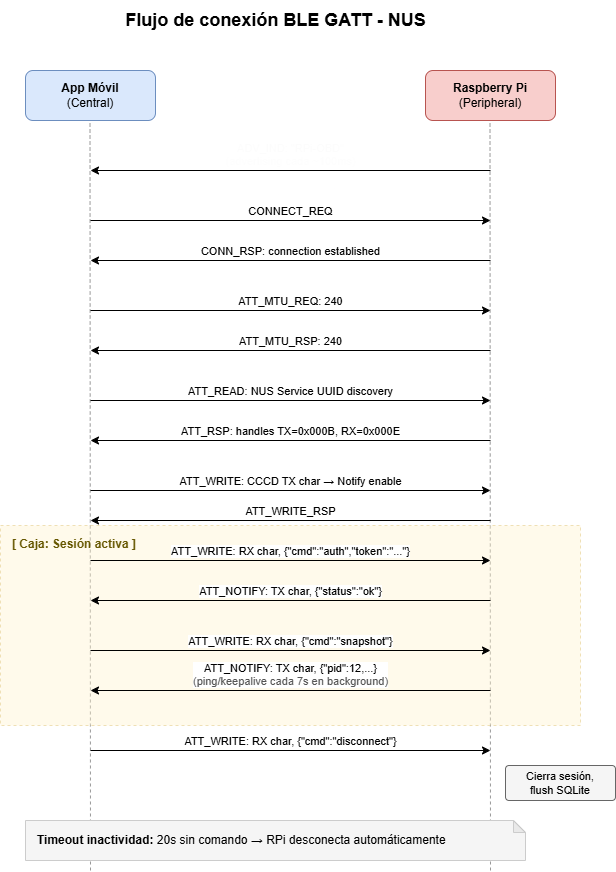
\includegraphics[width=0.8\textwidth]{Ilustraciones/ble_gatt_flow.png}
